\begin{question}
  \hspace*{\fill} [Note Maximale: 16]\par
  \medskip
  \noindent Soit la fonction $f(x) =\frac{x}{-2x^2 + 5x - 2}$, pour $-2 \le x \le 4$, $x \ne frac{1}{2}$, $x\ne2$\par
  \medskip
  \begin{center} % or flushleft or flushright
    \noindent Représentation graphique de $f$\par
    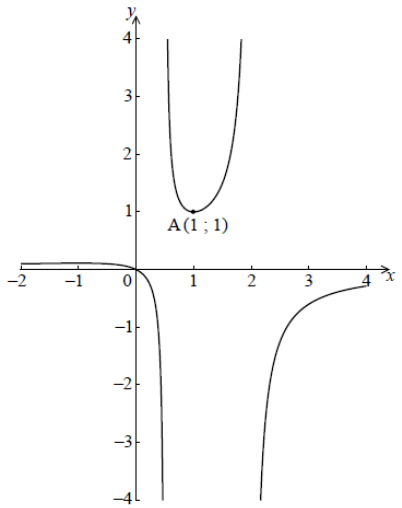
\includegraphics[scale=0.3]{figure_x7}\par
    \noindent La courbe a un minimum local en $A(1;1)$ et un maximum local en $B$\par
  \end{center} % or flushleft or flushright
  \begin{enumerate}[label=(\alph*)]
    \item Utilisez la règle de dérivation du quotient pour montrer que $f^\prime(x)=\frac{2x^2 - 2}{(-2x^2+5x-2)^2}$\hspace*{\fill} [6]
    \item À partir de là, trouvez les coordonnées de $B$.\hspace*{\fill} [7]
    \item Étant donné que la droite $y=k$ ne rencontre pas la courbe de $f$, trouvez les valeurs possibles de $k$.\hspace*{\fill} [3]
  \end{enumerate}
\end{question}
